\documentclass[11pt,a4paper,oneside]{scrartcl}
\usepackage{requiredPackages}
\usepackage{subfig}
\usepackage{cancel}
\usepackage[labelfont=bf]{caption}
\usepackage{booktabs}
\interfootnotelinepenalty=10000

\def\UrlBreaks{\do/\do-\do_}
\begin{document}
\begin{titlepage}
	\centering
	{\scshape\LARGE Ludwig-Maximilians-Universität \linebreak München \par}
	\vspace{1cm}
	{\scshape\Large Fortgeschrittenenpraktikum II \par Wintersemester 22/23 \par}
	\vspace{1.5cm}
	{\huge\bfseries \par  Gaußsche Strahlenoptik\par}
	\vspace{2cm}
	{\Large\itshape Guido Osterwinter und Jan-Philipp Christ \par}
	\vfill
	{\large München, den \today\par}
\end{titlepage}

\tableofcontents
\newpage
\section{Zielsetzung}
Die geometrische Optik liefert nur eine unzureichende Beschreibung von Laserstrahlen, da im Rahmen dieser der Wellencharakter des Lichtes gänzlich vernachlässigt wird. Deutlich wird dies insbesondere bei konvergenten Strahlen, die nach der geometrischen Optik in einen einzelnen Punkt zusammenlaufen würden, obwohl dies durch Beugungseffekte nicht zulässig ist. \\
Berücksichtigt man nun den Wellencharakter des Lichtes und das typischerweise gauß-förmige Intensitätsprofil eines Laserstrahls, führt dies zur Gaußschen Strahlenoptik. \\
Im ersten Teil des hier vorgestellten Versuchs soll es um das experimentelle Untersuchen charakteristischer Größen eines solchen Laserstrahls gehen. So wird die Strahltaille (Waist) senkrecht zur Ausbreitungsrichtung sowie der Strahlradius als Funktion der zur Ausbreitungsrichtung parallelen Koordinate untersucht.\\
Im zweiten Versuchsteil wird das Verhalten Gaußscher Strahlen in einem aus zwei gekrümmten halbdurchlässigen Spiegel bestehenden Resonator untersucht. Insbesondere wird auf die Transmissionsfunktion als Funktion des Spiegelabstandes eingegangen und beispielhaft die Finesse eines konfokalen Resonators bestimmt. 
\section{Theoretischer Hintergrund}
\subsection{Gaußstrahlen}
\subsubsection{Ideale Gaußstrahlen}
Die Darstellung in diesem Abschnitt stützt sich, sofern nicht anders angegeben, auf Abschnitt 1 aus \cite{versuchsanleitung}. \\
Für monochromatische Lichtfelder linearer Polarisation der Form 
\begin{equation}\label{E_vec}
\vec E(\vec x,t)=\vec e\cdot E(x,y,z)\cdot e^{i\omega t}
\end{equation}
wird die elektromagnetische Wellengleichung in homogenen Medien zu
\begin{equation}\label{wave_eq}
\left(\frac{\partial^2}{\partial x^2}+\frac{\partial^2}{\partial y^2}+\frac{\partial^2}{\partial z^2}+k^2\right)E(x,y,z)=0
\end{equation}
Breitet sich ein Lichtfeld entlang der z-Richtung aus, so vereinfacht sich die Ortsabhängigkeit der Amplitude in \ref{E_vec} zu 
\begin{equation}\label{E_ansatz}
E(x,y,z)=E_0X(x,z)Y(y,z)e^{-ikz}.
\end{equation}
Nun sind häufig nur Strahlen von Interesse, die der schon aus der geometrischen Optik bekannten paraxialen Näherung genügen. Dies umfasst Strahlen, die sich nah an der optischen Achse bewegen und mit dieser nur kleine Winkel einschließen. Somit verschwinden für solche Strahlen in guter Näherung die zweiten partiellen Ableitungen nach $z$, da diese, wenn sie nicht $0$ wären, ein \glqq Wegkrümmen\grqq\ des Strahls von der optischen Achse beschreiben würden.\\
Einsetzen von \ref{E_ansatz} in \ref{wave_eq} liefert mit $X\equiv X(x,z), Y\equiv Y(y,z)$:
\begin{align}
0&=\left(\frac{\partial^2}{\partial x^2}+\frac{\partial^2}{\partial y^2}+\frac{\partial^2}{\partial z^2}+k^2\right)E(x,y,z) \\ \quad&
=\left(\frac{\partial^2}{\partial x^2}+\frac{\partial^2}{\partial y^2}+k^2\right)E(x,y,z)+\partial_z\left(-ikE_0XYe^{-ikz}+E_0e^{-ikz}\partial_z(XY)\right) \\ \quad&
=\left(\frac{\partial^2}{\partial x^2}+\frac{\partial^2}{\partial y^2}+\cancel{k^2}\right)E(x,y,z)-\cancel{k^2E_0XYe^{-ikz}}-2ikE_0\partial_z(XY)e^{-ikz}\\ \quad& -ikE_0e^{-ikz}XY+E_0e^{-ikz}\underbrace{\partial_z^2(XY)}_{\approx 0}
\end{align}
Man überzeugt sich nun nach einmaligem Anwenden der Produktregel auf den Term mit $\partial_z$ schnell davon, dass für nicht-triviale $X,Y$ gelten muss:
\begin{equation}
\left(\frac{\partial^2}{\partial x^2}-2ik\frac{\partial}{\partial z}\right)X(x,z)=\left(\frac{\partial^2}{\partial y^2}-2ik\frac{\partial}{\partial z}\right)y(y,z)=0
\end{equation}
Lösungen hiervon sind die Hermite-Gaußschen $\mathrm{TEM}_{m,n}$ Moden. Dabei beschreiben $n,m\in\N$ die Anzahl von Knoten im axialen Intensitätsprofil in $x-$ respektive $y-$Richtung.\\
Die Stärke der Divergenz dieser Moden wird bestimmt durch den Waist $w_0$, der auch die sogenannte Rayleigh-Länge \begin{equation}\label{rayleigh} z_R\equiv \frac{\pi w_0^2n}{\lambda}\end{equation}festlegt. Der Strahlradius nimmt entlang der Ausbreitungsrichtung die folgende Form an ($z_0$ ist der Ort, an dem die Waist angenommen wird):
\begin{equation}
\label{transv_profil}
w(z)=w_0\sqrt{1+\frac{(z-z_0)^2}{z_R^2}}
\end{equation}
Wie sich herausstellt, beschreibt das Wertepaar $(w_0,z_R)$ und damit auch die Größe $q\equiv w_0+iz_R$ einen Gaußstrahl vollständig.\\
Wird nun ein optisches System durch eine Transfermatrix \begin{equation}
T\equiv\begin{bmatrix}
A& B\\
C & D
\end{bmatrix}
\end{equation}
beschrieben- zur Berechnung von Transfermatrizen für einige konkrete Systeme vergleiche beispielsweise \cite{demtröder_2}- so werden $w_0$ und $z_R$ gemäß dem sogenannten 'ABCD'-Gesetz für Gaußstrahlen transformiert:
\begin{equation}\label{ABCD-Gesetz}
q^\prime = \frac{Aq+B}{Cq+D}
\end{equation}
\subsubsection{Reale Gaußstrahlen}\label{Reale Gaußstrahlen}
Reale (Laser-)Strahlen lassen sich natürlich nur in einem gewissen Maße als ideale Gaußstrahlen beschreiben. Um dem Verhalten realer Gaußstrahlen Rechnung zu tragen, führt man die dimensionslose Beugungsmaßzahl $M^2$ ein (vgl. \cite{paschotta2016m2}). Es ist für Gaußstrahlen $M^2=1$ und allgemein $M^2\geq 1$. Ein realer Strahl weitet sich gemäß dem Zusammenhang
\begin{equation}\label{rayleigh_m2}
z_R=\frac{w_0^2\pi n}{\lambda}\cdot \frac1{M^2}
\end{equation}
schneller auf als ein idealer Gaußstrahl. Da nach Gleichung \ref{ABCD-Gesetz} $z_R$ nicht durch ideale optische Elemente wie Linsen verändert wird, ist auch $M$ invariant unter idealen optischen Elementen. Dieser Umstand wird später noch aufgegriffen.
\subsubsection{Beispiel für Anwendung des 'ABCD'-Gesetzes}
\image{Skizze_A1}{Fokussierung eines Gaußstrahls auf bestimmten Waist $w^\prime_0$}{1}{Skizze_Aufgabe_S7.png}
Gegeben zwei Konvexlinsen mit Brennweiten $f_1,f_2$ soll ein Laserstrahl, dessen Waist $w_0$ anfangs in der ersten Linse sei, auf den Waist $w_0^\prime$ präpariert werden. Hierfür soll der Abstand $d$ zwischen den beiden Linsen bestimmt werden.\\
Gegeben sind die Werte $w_0 = 1\ \mathrm{mm}$, $\lambda = 632.8\ \mathrm{nm}$, ${w'}_0 = 5 \mu \mathrm m$, $f_1 = 50\mathrm{mm}$, $f_2 = 100\ \mathrm{mm}$. Um hieraus $d$ zu bestimmen, betrachte man die Transfermatrix
\begin{equation}
\begin{bmatrix}
    1 & 0 \\
    -\frac{1}{f_2} & 1 
\end{bmatrix}
\cdot
 \begin{bmatrix}
    1 & d \\
    0 & 1 
\end{bmatrix}
\cdot
 \begin{bmatrix}
    1 & 0 \\
    -\frac{1}{f_1} & 1 
\end{bmatrix}
\,\,=\,\,
 \begin{bmatrix}
   1-\frac{d}{f_1} & d \\
    \frac{d-f_1-f_2}{f_1 f_2} & 1-\frac{d}{f_2} 
\end{bmatrix}
\equiv
 \begin{bmatrix}
   A & B \\
    C & D 
\end{bmatrix}
\end{equation}
Für die Umgebung, in der sich die Gaußstrahlen ausbreiten, sei in guter Näherung ein Brechungsindex von $n=1$ angenommen. Der Wert von $q$ in Abbildung \ref{Skizze_A1} ist dann
\begin{equation}
q \,\,=\,\, 0 + i \frac{\pi}{\lambda} w_{0}^2
\end{equation}
Gemäß dem 'ABCD'-Gesetz für Gaußstrahlen gilt damit für $q'$ in Abbildung \ref{Skizze_A1} Gleichung \ref{ABCD-Gesetz}.\\
Für $q'$ soll aber auch
\begin{equation}\label{Gl2}
q' \,\,=\,\, -f_2 + i \frac{\pi}{\lambda} {w'}_{0}^{2}
\end{equation}
gelten. Aus den Gleichungen \ref{ABCD-Gesetz} und \ref{Gl2} nach $d$ auf, erhält man für $d$ die definierende Gleichung
\begin{align}
\left( f_1 f_2 \frac{w_0}{{w'}_{0}} \right)^2 \,\,&=\,\, \left( f_1 f_2 - d f_1 \right)^2 + \left( d - f_1 - f_2 \right)^2 \cdot \left(\frac{\pi w_{0}^{2}}{\lambda} \right)^2\\ \quad&
\Rightarrow \,\,\,\, d \,\,=\,\, 35.14\ \mathrm{cm}
\end{align}
Eine analoge Rechnung bei $f_2\leftrightarrow f_1$ liefert mit $d=35.13\ \mathrm{cm}$ nahezu den identischen Wert.
\subsection{Optische Resonatoren}
Auch die Darstellung in diesem Abschnitt stützt sich, sofern nicht anders angegeben, auf Abschnitt 1 aus \cite{versuchsanleitung}. \\
Ein optischer Resonator ist ein Paar aus halbdurchlässigen Spiegeln, in Abhängigkeit von deren Krümmungsradien $R$ und Abstand $L$ zueinander Randbedingungen für die transmittierten Moden festgelegt werden. Es gilt für die Strahltaille:
\begin{equation}
w_0^2=\frac{\lambda}{\pi}\sqrt{\frac{L}{2}\left(R-\frac{L}{2}\right)}
\end{equation}
Im Versuch wird ein symmetrischer Resonator verwendet, bei dem die Waist in der Mitte der Spigel liegt und die beiden Spiegel dieselben Krümmungsradien haben. Da zudem $L\approx R$ sein soll, spricht man von einer konfokalen oder zumindest nah-konfokalen Anordnung.\\
Im Wesentlichen ist auch von einem Resonator mit gekrümmten Spiegeln eine derjenigen eines planaren Fabry-Perot-Resonators ähnliche Transmissionsfunktion zu erwarten mit dem Unterschied, dass die Phasendifferenz nach einem Durchlauf i.A. nicht mehr nur von der Geometrie des Resonators, sondern beispielsweise auch von der eingekoppelten Mode abhängt. \\
Eine charakteristische Größe eines Fabry-Perot-Resonators ist die Finesse $F$ die das Verhältnis aus dem freien Frequenzbereich (Abstand zwischen zwei Resonanzpeaks) und der FWHM-Breite eines Resonanzpeaks beschreibt:
\begin{equation}
F\equiv \frac{\Delta \omega_{\mathrm{FSR}}}{\Delta \omega_{\mathrm{FWHM}}}
\end{equation}
Andererseits kann man zeigen, dass, wenn die beiden Spiegel die Reflektivitäten $R_1$ und $R_2$ haben, die folgende Beziehung zwischen der Gesamtreflektivität $R\equiv \sqrt{R_1R_2}<1$ und $F$ gilt:
\begin{equation}\label{finesse_theor}
F= \frac{\pi\sqrt{R}}{1-R}
\end{equation}
\subsubsection{Aufbau des verwendeten Resonators}
\image{Skizze_A2}{Aufbau zum optischen Resonator (aus \cite{versuchsanleitung}, bearbeitet)}{.8}{Skizze_Aufgabe_S16.png}
\setcounter{figure}{3}
Damit sich im symmetrischen nah-konfokalen Resonator aus sphärischen Spiegeln eine stehende Welle bilden kann, soll die Waist des Gauß-Strahls mittig zwischen den beiden Spiegeln liegen. Betrachtet man den halbdurchlässigen Spiegel $\mathfrak{S}$, durch den der Gaußstrahl in den Resonator einfällt, als Linse der Dicke $b=6.35\ \mathrm{mm}$ und mit Krümmungsradien $R_1=\infty,R_2\equiv R=50\ \mathrm{mm}$, so kann unter Zuhilfenahme der Brechungsmatrix 
\begin{align}
B_R\equiv \begin{bmatrix}
1 & 0\\
\frac{n_1-n_2}{n_2\cdot R} & \frac{n_1}{n_2}
\end{bmatrix} 
\end{align}
an einer gekrümmten Ebene zwischen zwei Medien mit Brechungsindizes $n_1$ und $n_2$
nach \cite{dewiki:225621757} die Transfermatrix von $\mathfrak{S}$ bestimmt werden:
\begin{align}
T & \equiv
\begin{bmatrix}
A & B\\
C & D 
\end{bmatrix} 
\equiv
\begin{bmatrix}
1 & 0\\
\frac{n-1}{|R|} & \frac{n}{1}
\end{bmatrix} 
\cdot
\begin{bmatrix}
1 & b\\
0 & 1
\end{bmatrix} 
\cdot
\begin{bmatrix}
1 & 0\\
\frac{1-n}{n\cdot \infty} & \frac{1}{n}
\end{bmatrix} 
\\ \quad& = \begin{bmatrix}
1 & \frac{b}{n}\\
\frac{n-1}{R} & 1+\frac{b(n-1)}{nR}
\end{bmatrix}
\end{align}
Im Resonator geben die Randbedingungen vor, dass $w_0^\prime=\sqrt{\frac{\lambda}{\pi}\sqrt{\frac{d}{2}\left(R-\frac{d}{2}\right)}}$ gilt, wodurch insbesondere $q^\prime\equiv z^\prime+iz_R^\prime$ festgelegt wird. Damit lässt sich auf $q=z+iz_R$ außerhalb des Resonators, also vor dem Einkoppeln des Strahls in den Resonator, schließen:
\begin{align}
\ref{ABCD-Gesetz}& \iff q = \frac{Dq^\prime-B}{A-Cq^\prime}\\ & \Rightarrow z_R=\Im{q}%=\Im{\frac{D\cdot (z^\prime+iz_R^\prime)-B}{A-C\cdot(z^\prime+iz_R^\prime)}}\\ \quad&=\Im{\frac{D\cdot ((z^\prime+iz_R^\prime)-B)(A-C\cdot(z^\prime-iz_R^\prime))}{(A-Cz^\prime)^2+C^2z_R^{^\prime 2}}}
=\frac{ADz_R^\prime-BCDz_R^\prime}{(A-Cz^\prime)^2+C^2z_R^{^\prime 2}}
\end{align}
Analog folgt 
\begin{equation}
z=\frac{ADz^\prime+BCDz^\prime-ABD-CDz^{\prime 2}-CDz_R^{\prime 2}}{(A-Cz^\prime)^2+C^2z_R^{^\prime 2}}
\end{equation}
Da beide Spiegel denselben Krümmungsradius haben, müssen resonante Strahlen ihren Waist in der Mitte der beiden Spiegel haben. $z^\prime$ ist also gerade der halbe Abstand $d=45\ \mathrm{mm}$ der beiden Spiegel. Die Wellenlänge $\lambda=632.8\ \mathrm{nm}$ ist die Wellenlänge des verwendeten HeNe-Lasers. \\
Einsetzen liefert zunächst
\begin{equation}
w_0^\prime = 70.08\ \mu\mathrm m\Rightarrow z_R^\prime = \frac{\pi w_0^{\prime 2}}{\lambda} = 2.49\ \mathrm{cm}
\end{equation}
 $z^\prime$ ist der negative halbe Abstand der beiden halbdurchlässigen Spiegel, da mittig zwischen diesen der waist des Strahls liegt. \\
Damit ergibt sich für die Strahlparameter außerhalb des Resonators (d.h. vor dem Einkoppeln des Strahls in den Resonator) durch Einsetzen
\begin{equation}
z_R = 1.57\ \mathrm{cm},\ z = -2.59\ \mathrm{cm}
\end{equation}
Der Fokus ist also scheinbar um $\Delta z\equiv z-z^\prime = -3.4\ \mathrm{mm}$ verschoben. \\
Dass der Fokus der Linse für Modenanpassung bei der Versuchsdurchführung direkt auf das \emph{geometrische} Zentrum des Resonators gelegt wurde, ist also in guter Näherung eine valide Herangehensweise, da die ebenfalls auf einem verschiebbaren Tisch montierte Linse beim Feinjustieren ohnehin noch etwas verschoben werden kann.
\section{Versuchsdurchführung}
\subsection{Materialliste}
Es wurden die folgenden Utensilien verwendet:
\begin{itemize}
\item ein HeNe-Laser ($\lambda=632.8\ \mathrm{nm}$, $P\sim 1\mathrm{mW}$)
\item zwei Photodioden mit Eigenwiderstand $R=100\ \mathrm{k\Omega}$
\item ein Oszilloskop
\item eine elektrische Schaltung, die das Verhältnis aus zwei (Eingangs-)Spannungen liefert
\item Funktionsgenerator
\item zwei konvexe Linsen mit $f=50\ \mathrm{mm},\ f=100\ \mathrm{mm}$
\item Single-Mode Glasfaser FS-SN-3224-FC, Multi-Mode-Glasfaser FS-SC-6324 sowie zwei Faserkoppler
\item durch Piezo-Elemente verstellbarer Resonator bestehend aus Spiegelpaar mit Krümmungsradien $R=100\ \mathrm{mm}$
\item Verschiebetisch mit Mikrometerschraube und Rasierklinge
\end{itemize}
\subsection{Bestimmung der Laserleistung und der Hintergrundhelligkeit}
\image{Skizze_aufwaermen}{Aufbau zur Bestimmung der Laserleistung (aus \cite{versuchsanleitung})}{.6}{Aufwaermen_Skizze.jpg}
Zunächst sollte die Lichtleistung des verwendeten HeNe-Lasers bestimmt werden. Dafür wurde ein Aufbau nach Abbildung \ref{Skizze_aufwaermen} benutzt: Der Laserstrahl traf nach einem Strahlteiler und einem justierbaren Spiegel auf eine Konvexlinse, die den Strahl auf die aktive Fläche der Photodiode fokussierte. Es wurde die Spannung über der Photodiode, die einen Widerstand von $R=100\ \mathrm{k}\Omega$ verfügt, gemessen und der Wert $U_{L,\mathrm{hell}}=(9.94\pm 0.02)\ \mathrm V$ für die Spannung im hellen Raum mit Laser, der Wert $U_{R,\mathrm{hell}}=(0.0505\pm 0.001)\ \mathrm V$ ohne Laser im hellen Raum, der Wert  $U_{L,\mathrm{dunkel}}=(9.95\pm 0.02)\ \mathrm V$ mit Laser im verdunkelten Raum und der Wert  $U_{R,\mathrm{dunkel}}=(1.6\pm 0.2)\ \mathrm{mV}$ ohne Laser im verdunkelten Raum aufgenommen.\\
Es erscheint paradox, dass $U_{L,\mathrm{hell}}<U_{L,\mathrm{dunkel}}$. Da aber die Abweichung der beiden Werte kleiner ist als die Unsicherheiten der Messwerte, ist diese Abweichung von der Erwartung $U_{L,\mathrm{hell}}>U_{L,\mathrm{dunkel}}$ als durch statistische Schwankungen bedingt anzusehen.
 
\subsection{Einkoppeln des Laserstrahls}
\begin{figure}[H]
\setcounter{imEnv}{1}
    \centering
    \subfloat[Single-Mode]{
        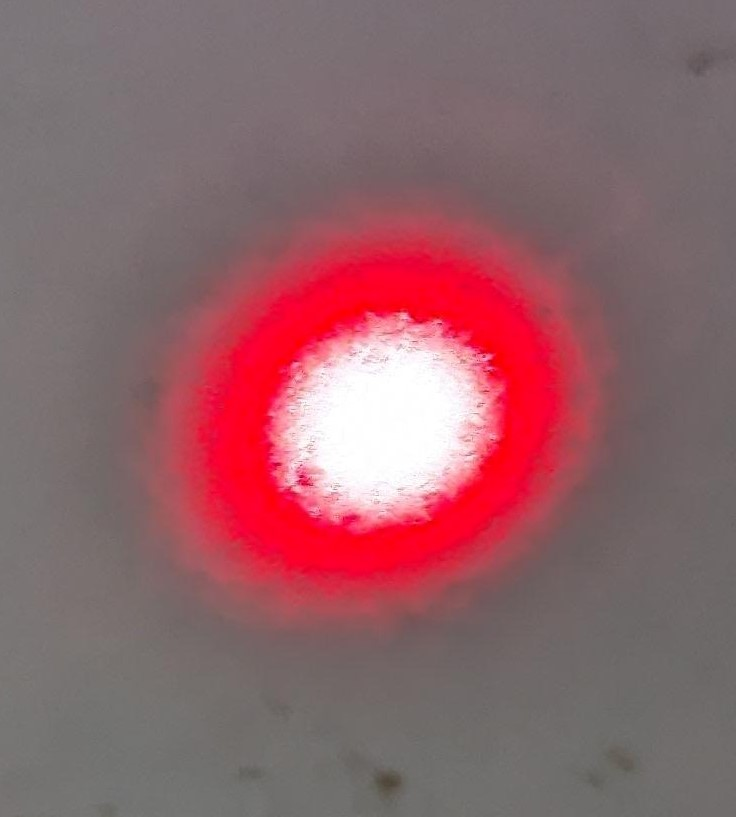
\includegraphics[width=0.28\textwidth]{Bilder/single_mode_fiber.jpg}
    }
  \subfloat[Multi-mode]{
        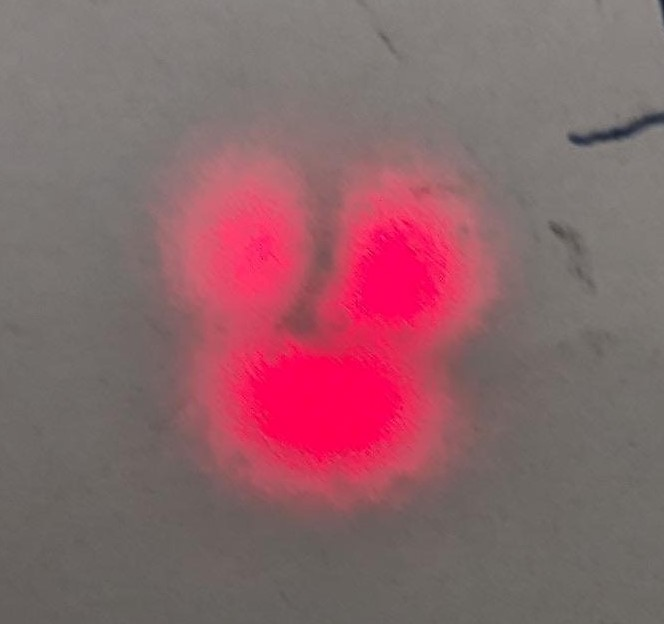
\includegraphics[width=0.3294\textwidth]{Bilder/multi_mode_fiber.jpg}
    }\\
   \caption{Transmittierte Moden nach Glasfasern hinter $f=50\ \mathrm{mm}$ Linse}
    \label{FotostreckeGlasfasern}
\end{figure}
\subsection{Untersuchung eines Gaußschen Laserstrahls}

\subsubsection{Vermessung der Strahltaille}\label{Durchführung Vermessung der Strahltaille}
\setcounter{imEnv}{4}
\image{Skizze_Strahltaille}{Aufbau zum Vermessen der Strahltaille (aus \cite{versuchsanleitung})}{.6}{Skizze_Razor.jpg}
Es wurde das Strahlprofil kurz hinter dem Faserkoppler vermessen, indem ein auf einem verschiebbaren Tisch positioniertes Rasiermesser so platziert wurde, dass es einen Teil des Lichtstrahles blockte. Das transmittierte Licht konnte dann nach \ref{Skizze_Strahltaille} auf die Photodiode fokussiert werden. Es wurde nicht direkt die Spannung der Photodiode gemessen, sondern eine Spannung proportional zum Quotienten von der Spannung der Photodiode aus \ref{Skizze_Strahltaille} und der Spannung einer weiteren Photodiode, auf die über einen Strahlteiler ein zur Ausgangsleistung des Lasers proportionale Strahlungsleistung fiel. Das Bilden des Quotienten wurde über eine elektrische Schaltung realisiert. Idealerweise bereinigt die Quotientenbildung die Messergebnisse so von kleinen Schwankungen im Laseroutput.\\
Gemessen wurde damit aber insbesondere weiterhin eine Spannung, die zur Photodiodenspannung, nach dem Ohmschen Gesetz damit auch zum Photostrom und entsprechend auch zur Strahlungsleistung proportional ist. Aufgenommen wurden die in \plotref{coll_z_75} eingezeichneten Messwerte. Beim Aufnehmen dieser wurde darauf geachtet, dass in dem Bereich, in dem kleine Verschiebungen in der Klingenposition relativ große Änderungen in der gemessenen Spannung nach sich ziehen, der Abstand zwischen benachbarten Messpunkten ausreichend klein war. Erschwert wurde das Ablesen durch die starken Schwankungen auf der Multimeteranzeige, die weit über die typischerweise zu erwartende Messunsicherheit eines Multimeters hinaus gingen. Auf Basis dieser Schwankungen wurde bei jedem Messwert die Unsicherheit in der Spannung geschätzt.
%und daraus folgt
%\begin{equation}
%\frac{w_1^2}{w_2^2}=\frac{1+z_1^2/z_R^2}{1+z_2^2/z_R^2}\Rightarrow z_R=\sqrt{\frac{z_1^2-\frac{w_1^2}{w_2^2}z_2^2}{\frac{w_1^2}{w_2^2}-1}}.
%\end{equation}
%Mithilfe des so bestimmten Wertes kann $w_0$ bestimmt werden. 
%\begin{equation}
%w_0=\frac{w_i}{\sqrt{1+\frac{z_i^2}{z_R^2}}},\ i\in\{1,2 \}
%\end{equation}
\subsubsection{Abschätzung der Parameter des kollimierten Laserstrahls}
In gleicher Weise wie in \ref{Durchführung Vermessung der Strahltaille} wurde nun für $z=150\ \mathrm{mm},\ 250\ \mathrm{mm},\ 350\ \mathrm{mm}$ ($z=0$ beim Faserkoppler) jeweils der entsprechende Strahlradius $w(z)$ bestimmt. Die Messwerte sind in \plotref{coll_z_150} bzw. \plotref{coll_z_250} sowie \plotref{coll_z_350} einschließlich ihrer Fehlerbalken eingetragen. Für die Unsicherheiten in $z$ wurde ein Fehler von $\Delta z=1\ \mathrm{mm}$ bedacht, der aber angesichts der erheblich größeren Fehler in der Spannungsmessung vernachlässigbar ist und im Folgenden vernachlässigt werden kann.\\
Qualitativ konnte beobachtet werden, dass sich der Strahl im Messbereich weder stark aufweitete noch verengte, was der Erwartung, dass den Faserkoppler ein kollimierter Strahl verlässt, entspricht. Sichtbar gemacht werden konnte dies durch das Bewegen eines Blatt Papiers entlang des Messbereichs.
\subsubsection{Vermessung des Strahlprofils hinter einer Konvexlinse}
Nun wurde eine Konvexlinse der Brennweite $f=100\ \mathrm{mm}$ in den Strahl gestellt. Diese führte zu einer deutlich schnelleren Aufweitung des Strahls im Vergleich zu dem Strahl, der den Faserkoppler verlässt, was erneut durch das Bewegen eines Blatt Papiers entlang des Strahls sichtbar gemacht werden konnte. \\
Für $z=50\ \mathrm{mm},75\ \mathrm{mm},100\ \mathrm{mm},125\ \mathrm{mm},175\ \mathrm{mm}, 250\ \mathrm{mm}$ wurde der Strahldurchmesser $w(z)$ bestimmt, wobei $z$ von der $f=100\ \mathrm{mm}$ Linse aus gemessen wird. Das Vorgehen zum Bestimmen der Strahlradien für ein festes $z$ ist identisch zum Vorgehen in Abschnitt \ref{Durchführung Vermessung der Strahltaille}.
\subsection{Optischer Resonator}

\subsubsection{Justieren und Bestimmen der Transmissionsfunktion}
\setcounter{figure}{5}
\begin{figure}[H]
    \centering
    \subfloat[gestörte Transmissionsfunktion]{
        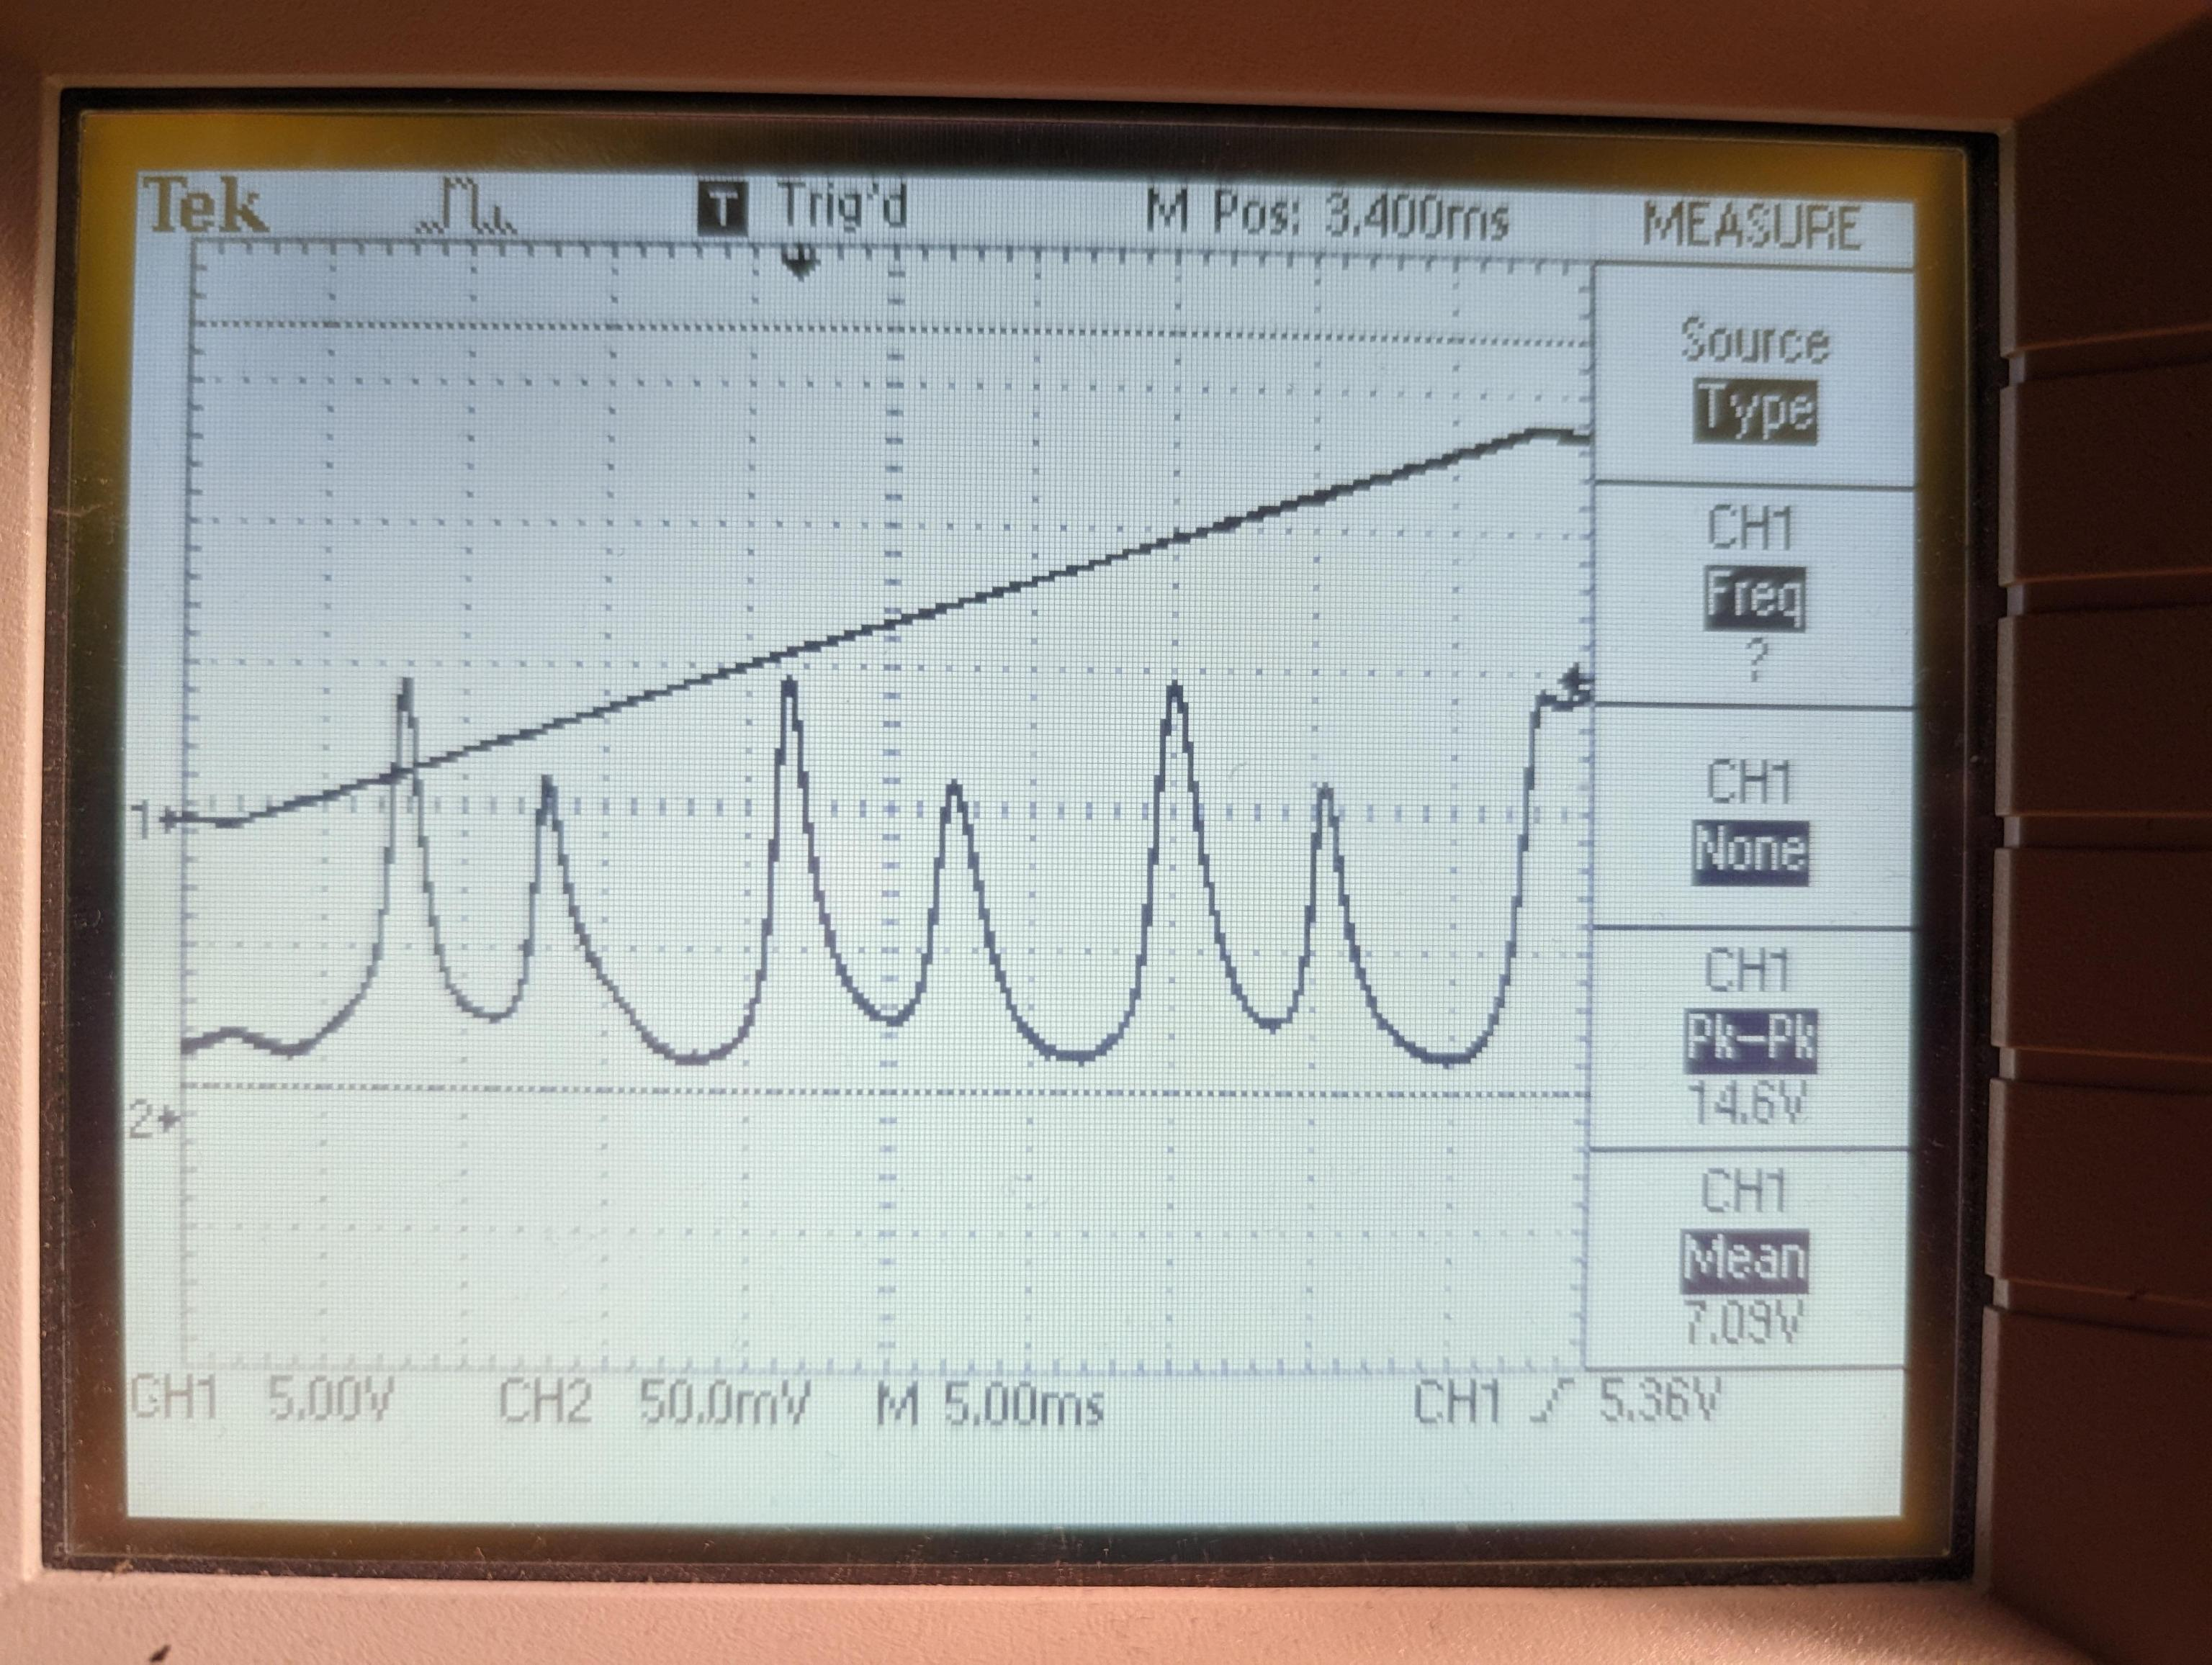
\includegraphics[width=0.4\textwidth]{Bilder/Osc_disturbed.jpg}
    }
  \subfloat[ungestörte Transmissionsfunktion]{
        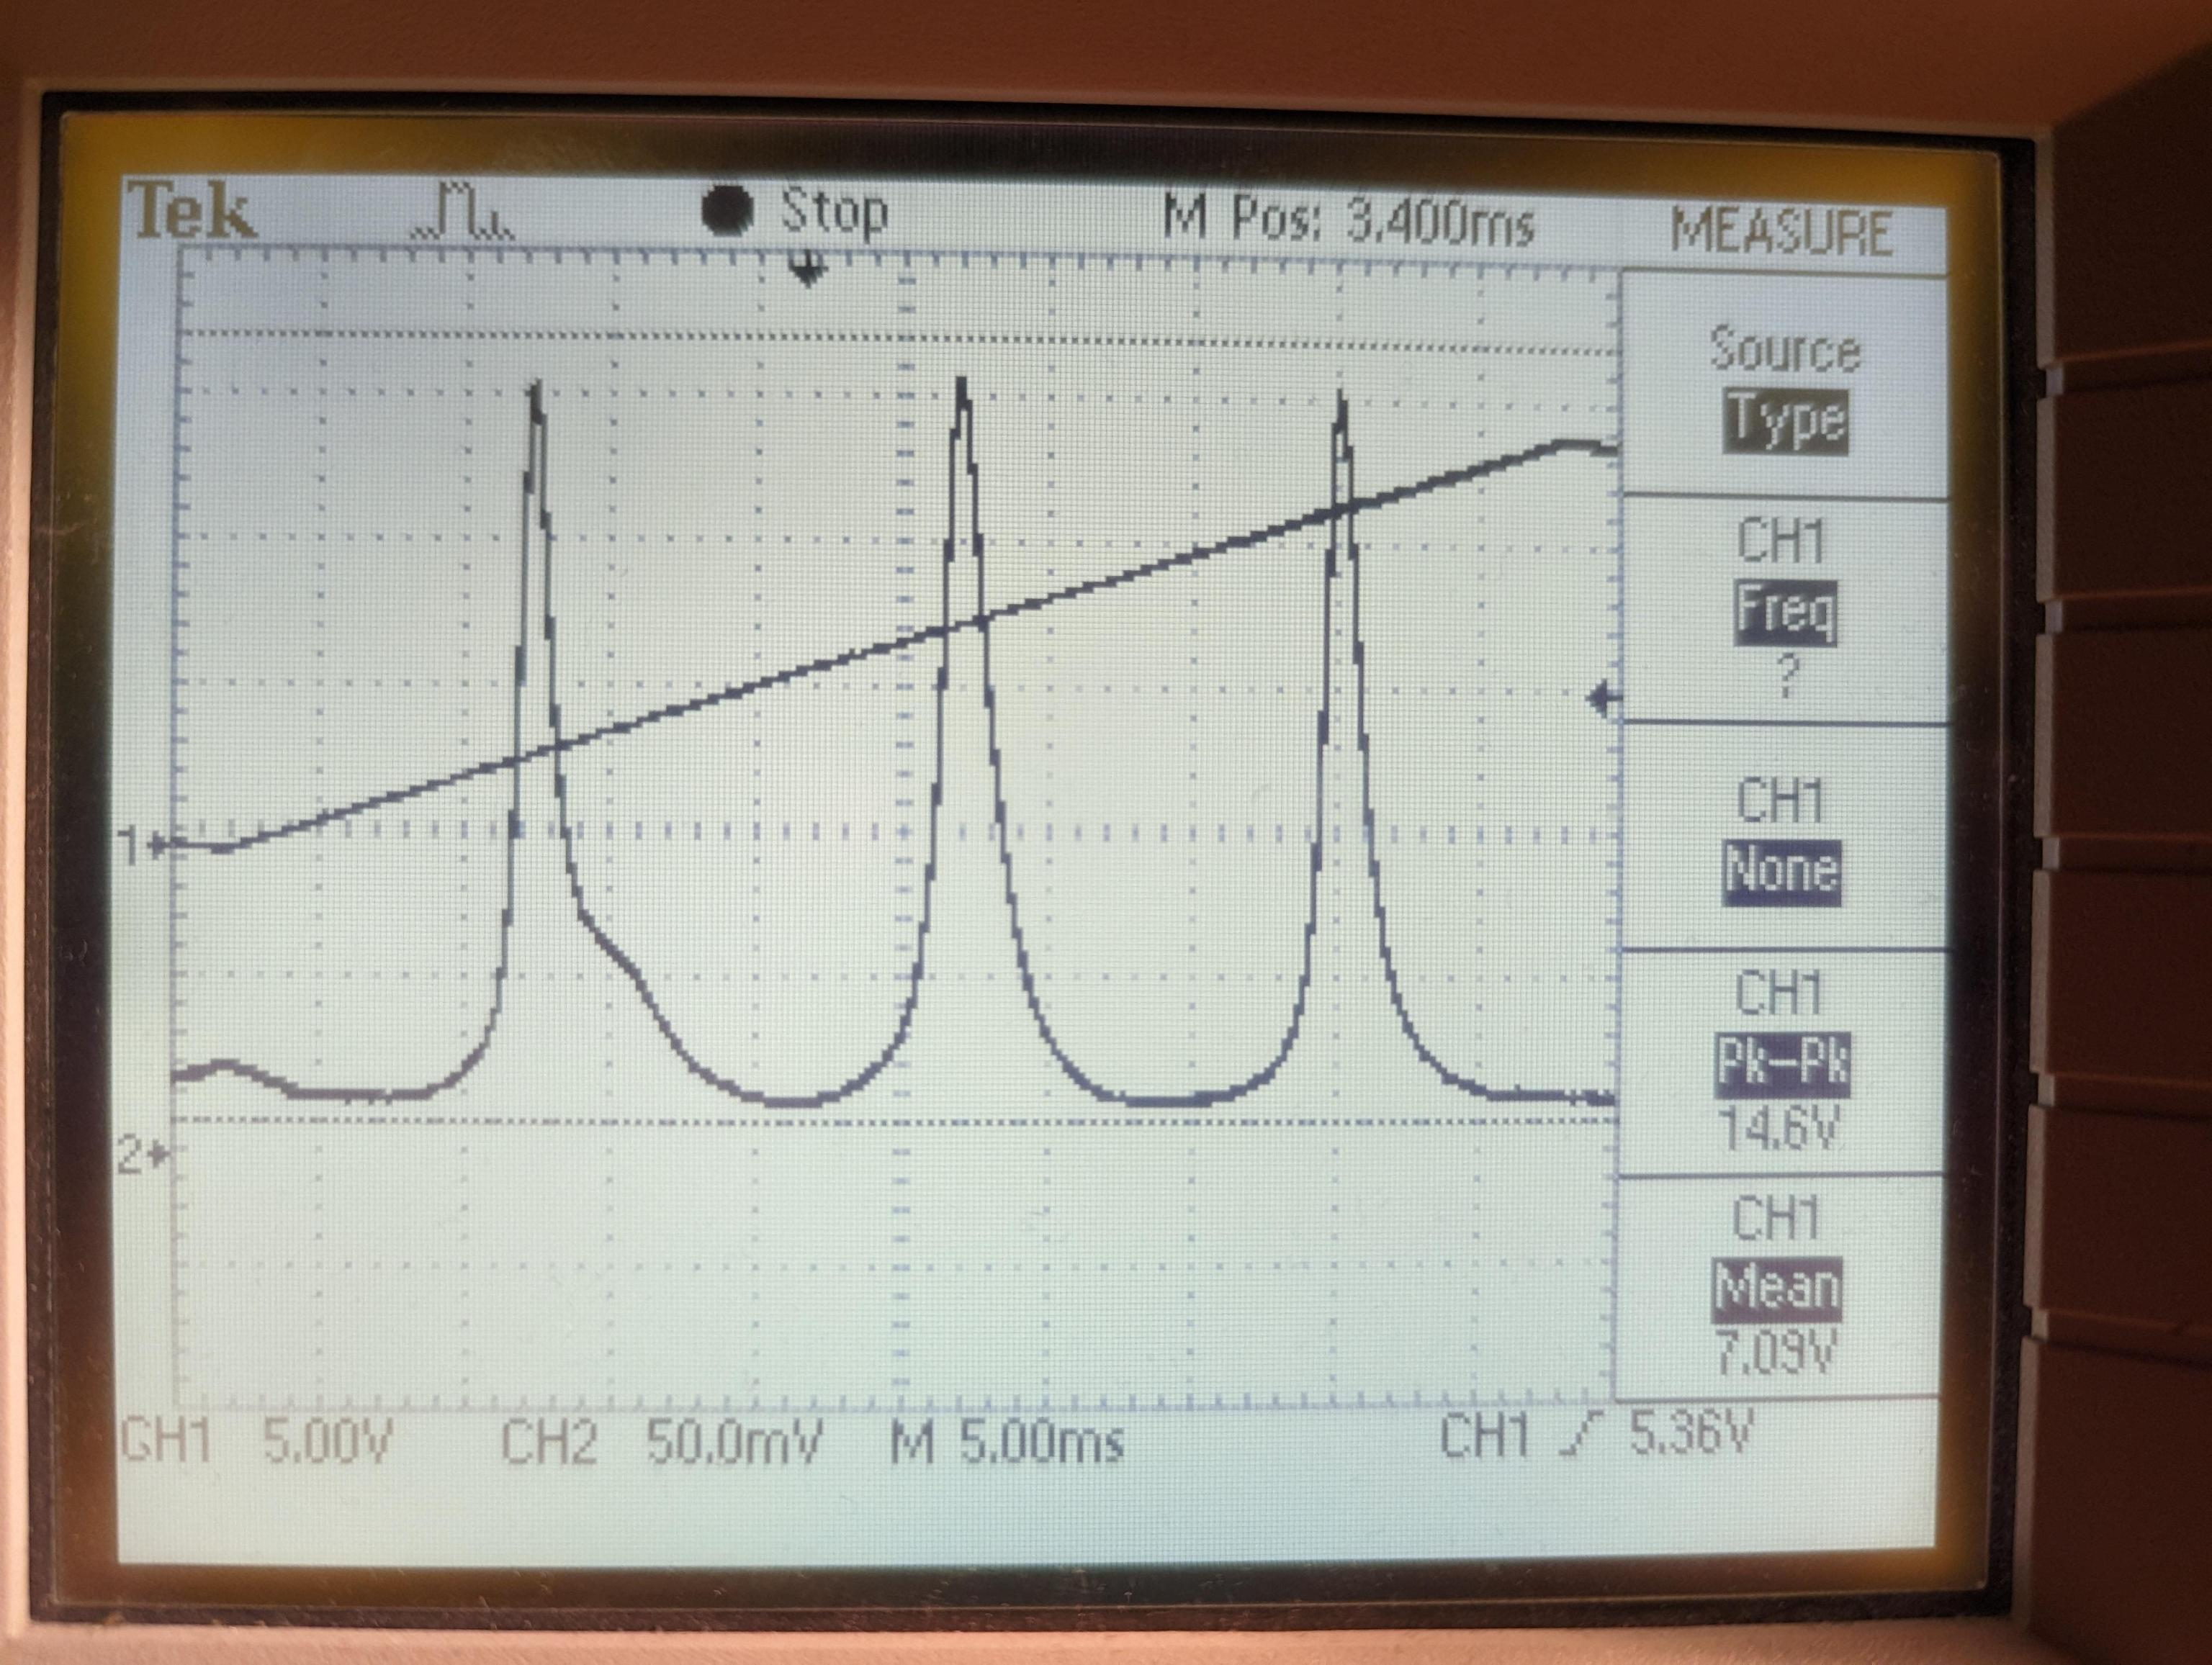
\includegraphics[width=0.4\textwidth]{Bilder/Osc_nice.jpg}
    }\\
   \caption{Transmissionsfunktion des konfokalen Resonators}
    \label{FotostreckeTransmissionsfunktion}
\end{figure}
%Berücksichtige nun die Linse zur Modenanpassung und deren Abstand $\mathfrak{d}$ zum Resonator.

\section{Ergebnisse und Diskussion}
\subsection{Bestimmung der Laserleistung und der Hintergrundhelligkeit}

Geht man bei der Photodiode von einem Quantenwirkungsgrad $\eta=75\%$ aus, so ergibt sich unter Ausnutzung der Propotionalität von Photostrom und einfallender Lichtleistung die von Photonen erzeugte Anzahl freier Elektronen und daraus der folgende Zusammenhang zwischen der Laserleistung $P$ und der gemessenen Spannung:
\begin{equation}\label{P_diode}
P=\frac{hcU}{e\lambda\eta R}
\end{equation}
Dabei bezeichnet $h$ das Plancksche Wirkungsquantum, $e$ die Elementarladung, $c$ die Lichtgeschwindigkeit und $\lambda$ die mittlere Wellenlänge des einfallenden Lichtes. Beim Laser kann $\lambda_L=632.8\ \mathrm{nm}$ als fehlerfrei angenommen werden. Bei der Hintergrundhelligkeit wird $\lambda_R=(600\pm 100)\ \mathrm{nm}$ gesetzt.
Damit ergeben sich die folgenden Werte:\\
\begin{table}[H]
\centering
\begin{tabular}{@{}lllll@{}}
\toprule
                        & $\lambda$   & $P [\mathrm{mW}]$  & $\Delta P[\mathrm{mW}]$ &  \\ \midrule
mit Laser, heller Raum  & $\lambda_L$ & $0.2597$           & $0.0006$                &  \\
mit Laser, dunkler Raum & $\lambda_L$ & $0.2599$           & $0.0006$                &  \\
ohne Laser, heller Raum   & $\lambda_R$ & $1.4\cdot 10^{-3}$ & $0.3\cdot 10^{-3}$      &  \\
ohne Laser, dunkler Raum & $\lambda_R$ & $42\cdot 10^{-6}$  & $6\cdot10^{-6}$         &  \\ \bottomrule
\end{tabular}
\caption{Lichtleistungen im hellen/ dunklen Raum, mit/ ohne Laser}
\end{table}
Die Unsicherheiten wurden mit der MinMax-Methode abgeschätzt.\\
Es kann festgehalten werden, dass ein Vernachlässigen der Hintergrundstrahlung bei den anderen Teilversuchen gerechtfertigt ist, da während der Versuchsdurchführung im abgedunkelten Raum gearbeitet wurde. Die Werte für die Leistung des Lasers erscheinen realistisch, da die Sollleistung des Lasers $1\ \mathrm{mW}$ beträgt und am Strahlteiler, an der Linse und am Spiegel Verluste durch Absorption oder Sekundärreflexionen auftreten.\\
Ferner kann die Intensität an der Tischoberfläche berechnet werden, indem die aktive Fläche der Photodiode auf $A=(3\pm1)^2\mathrm{mm}^2$ geschätzt wird. Folglich ergibt sich mit $I=\frac{P_{R,\mathrm{hell}}}{A}=(0.15\pm0.09)\frac{\mathrm{W}}{\mathrm m^2}$ ein ungenauer, aber realistisch erscheinender Wert. \\
Eine Verbesserung der Messgenauigkeit Laserleistung könnte durch Berücksichtigen der verschiedenenen des einfallenden Wellenlängenspektrums, das in guter Näherung dem der Sonne gleichen sollte, erzielt werden. Für die Bestimmung der Intensität trägt die Unsicherheit der aktiven Diodenfläche substanziell bei, die nach Ausbauen der Diode aus ihrem Gehäuse mit einer Schieblehre sehr genau bestimmt werden könnte.
\subsection{Einkoppeln des Laserstrahls}
\subsection{Untersuchung eines Gaußschen Laserstrahls}
\subsubsection{Vermessung der Strahltaille}\label{Auswertung Vermessung der Strahltaille}
Die gemessene Lichtleistung ist 
\begin{align}
P(x)&=\int_{-\infty}^\infty \mathrm dy^\prime \int_x^\infty \mathrm dx^\prime I_0\cdot\mathrm{exp}\left(-\frac{2(x^\prime-x_0)^2}{w^2}-\frac{2(y^\prime-y_0)^2}{w^2}\right) \\ \quad& = \sqrt{\frac{\pi}{2}}wI_0\int_x^\infty \mathrm dx^\prime \mathrm{exp}\left(-\frac{2(x^\prime-x_0)^2}{w^2}\right) \undereq{CAS}\hdots \\ \quad& =I_0\sqrt{\frac{\pi}{8}}w\cdot\left(\mathrm{erf}\left(\frac{\sqrt{2}}{w}(x_0-x)\right)+1\right)\\ \quad& \equiv \mathfrak{P}_0\cdot\left(\mathrm{erf}\left(\frac{\sqrt{2}}{w}(x_0-x)\right)+1\right)
\end{align}
Entsprechend können die Messdaten durch Anpassung der Parameter $(\mathfrak P_0,w,x_0)\in \R\setminus\{0\}\times\R^+\times\R$ gefittet werden. Da aber $U(z)\sim P(z)$, liefert die Anpassung an die Spannung mit $\mathfrak P_0\rightarrow U_0$ einen identischen Wert für den Strahlradius $w$.
Es ergibt sich \plotref{coll_z_75}. Qualitativ erkennt man, dass insbesondere der Bereich nahe um den Strahlmittelpunkt, also nahe $x_0$, sehr gut durch die Fitkurve beschrieben wird. Ein Messwert sticht heraus, da dessen Fehlerbalken die Regressionskurve nicht schneidet. Denkbar ist ein Fehler beim Abmesen oder Notieren des Wertes oder ein unbedachtes Anschalten des Raumlichtes während der betreffenden Messung. Da es sich nur um einen einzigen Messwert handelt, ist nicht davon auszugehen, dass er die Fitparameter signifikant beeinflusst hat. \\
Man erhält für den Strahldurchmesser mit $w(z=75\ \mathrm{mm})=(1.33\pm0.17)\ \mathrm{mm}$ einen Wert, der im Vergleich mit der Austrittsöffnung beim Faserkoppler realistisch erscheint.
\subsubsection{Abschätzung der Parameter des kollimierten Laserstrahls}\label{Auswertung Abschätzung der Parameter des kollimierten Laserstrahls}
Analog zu \ref{Auswertung Vermessung der Strahltaille} erhält man für die verschiedenen $z$ die korrespondierenden Strahldurchmesser $w(z)$, wobei $z$ weiterhin vom Faserende gemessen aus wurde. Es sei auf die Plots \ref{coll_z_75}, \ref{coll_z_150}, \ref{coll_z_250} und \ref{coll_z_350} verwiesen. Allen ist die qualitativ gute Beschreibung der Messwerte durch die jeweilige Regressionskurve gemein, was sich in einer geringen relativen Unsicherheit im Fitparameter $w$ (Strahldurchmesser) zeigt.\\
Es gilt dann für allgemeine reale Gaußstrahlen
\begin{equation}\label{w(z)}
w(z)=w_0\sqrt{1+\frac{(z-z_0)^2}{z_R(w_0,\lambda,M)^2}}=\sqrt{w_0^2+\frac{(z-z_0)^2\lambda^2M^4}{\pi^2n^2w_0^2}}
\end{equation}
gemäß Beziehung \ref{rayleigh_m2} und Gleichung \ref{transv_profil}, womit man \plotref{coll_z} erhält: 
\plot{coll_z}{Strahlprofil des kollmierten Strahls}{1}{Messdaten Errorfunktion/w_z_data_coll.pdf}
Es fällt auf, dass die Regressionkurve die vier Messpunkte im Rahmen deren Messungenauigkeiten gut beschreibt. Jedoch sind die Standardabweichungen der Fitparameter $z_0$ und $M$ sehr groß, was visuell am breiten 1$\sigma-$Fehlerstreifen deutlich wird. Ferner ist der ermittelte Wert für $M$ weit über der für HeNe-Laser typischen Beugungsmaßzahl von nahe 1 (vgl. \cite{paschotta2008beam}), und der Strahl würde entgegen der Erwartung, dass ein nahezu kollimierter Strahl vorliegt, nach \plotref{coll_z} relativ stark fokussiert sein. Dies legt nahe, dass in \plotref{coll_z} Overfitting beobachtet werden kann, da die drei freien Parameter eine exakte Beschreibung von drei beliebigen und eine genaue Beschreibung von vier Messwerten zulassen, und dass die Kurve in \plotref{coll_z} den Sachzusammehang nicht physikalisch sinnvoll beschreibt.\\
Setzt man nun $M=1$ fest, so kann nach \ref{w(z)} eine Anpassung in $w_0,z_0$ vorgenommen werden. Warum ein Festsetzen von $M=1$ gerechtfertigt ist, wird in Abschnitt \ref{Auswertung Vermessung des Strahlprofils hinter einer Konvexlinse} deutlich werden.
\plot{coll_z_without_M2}{Strahlprofil des kollmierten Strahls bei $M=1$}{1}{Messdaten Errorfunktion/w_z_data_coll_without_M2.pdf}
Es wird klar, dass bei festem $M$ die Messwerte am besten durch den in guter Näherung linearen Teil von $w(z)$ für $\frac{(z-z_0)^2}{z_R^2}\leq1$ beschrieben werden. Die optimale Kurve zeigt einen beinahe konstanten Kurvenverlauf, der für einen kollimierten Strahl zu erwarten wäre. Da (nahezu) konstante Funktionen (nahezu) invariant unter Verschiebungen entlang der Abszisse sind, hat der Fitparameter $z_0$ in \plotref{coll_z_without_M2} eine sehr große Unsicherheit. Die kleinere, aber immer noch große, relative Unsicherheit von $w_0$ lässt sich auf die geringe Zahl an Messwerten und deren starke Streuung um die optimale Kurve zurückführen. Bei zukünftigen Durchführungen eines solchen Experiments ist also ein Aufnehmen von $n>4$ Messwerten empfehlenswert. Mehrere Messwerte würden auch dabei helfen, zu klären, ob eher \plotref{coll_z} oder \plotref{coll_z_without_M2} den physikalischen Zusammenhang besser beschreibt. Denn, wie bereits diskutiert, ist \plotref{coll_z} bei Berücksichtigung des Versuchsaufbaus nicht sinnvoll, andererseits ist die Streuung der Messwerte um die optimale Kurve in \plotref{coll_z_without_M2} sehr groß. Dies könnte mehrere Ursachen haben:
\begin{itemize}
\item (Temperaturbedingte) Leistungsschwankungen im Laser trotz der Bereinigung der Messungen durch das Aufnehmen einer Referenzspannung. Als das Fenster im Versuchszimmer zu Beginn der Versuchsdurchführung geöffnet war, unterlag die Raumtemperatur der Variabilität der Außentemperatur, welche mit zunehmender Zeit abnahm. Nachdem das Fenster im Versuchsverlauf geschlossen wurde, ist von einer allmählichen Erwärmung im Zimmer auszugehen. 
\item versehentliches Verrücken der Linse vor der Photodiode oder der Photodiode selbst zwischen zwei Messungen (durch Anstoßen)
\item Verschieben der Glasfaser. Ein Bewegen der Glasfaser kann eine veränderte transmittierte Leistung zur Folge haben (wenn auch der Effekt bei der Multi-Mode-Faser stärker als bei der Single-Mode-Faser zu beobachten war)
\end{itemize}
Letztlich kann nur ein Aufnehmen von weiteren Messwerten die entstandenen Unklarheiten klären.\\
Da aber $w_0$ aus \plotref{coll_z} und \plotref{coll_z_without_M2} im Rahmen ihrer Unsicherheiten übereinstimmen, kann abschließend $w_0=(1.0\pm0.7)\ \mathrm{mm}$ und damit ein Wert, der nicht viel mehr als die Größenordnung der Waist des kollimierten Strahls aussagt, festgehalten werden. 
\subsubsection{Vermessung des Strahlprofils hinter einer Konvexlinse}\label{Auswertung Vermessung des Strahlprofils hinter einer Konvexlinse}
Wie auch im vorhergehenden Abschnitt, kann nach \ref{w(z)} eine Anpassung der Messdaten gewonnen werden. 
\plot{div_z}{transversales Strahlprofil hinter $f=100\ \mathrm{mm}$ Linse}{1}{Messdaten Errorfunktion/w_z_data_div.pdf}
Das Betrachten von \plotref{div_z} zeigt einerseits, dass die Regressionskurve die Messdaten qualitativ gut zu beschreiben vermag, andererseits machen die große Unsicherheit in den Fitparametern $w_0$ und $M$ sowie der damit einhergehend sehr breite $1\sigma-$Fehlerstreifen klar, dass die Aussagekraft der optimalen Fitparameter als gering einzustufen ist. Immerhin kann festgehalten werden, dass $M=1.4\pm0.9$ im Rahmen der Messunsicherheiten mit der Beugungsmaßzahl eines idealen Gaußstrahls übereinstimmt. Die Aussagekraft von dem hier gewonnen Wert für $M$ ist höher als dem in \plotref{coll_z} bestimmten Wert, da die Datengrundlage in \plotref{div_z} größer ist. Weil nach der Bemerkung in \ref{Reale Gaußstrahlen} $M$ durch das Einführen einer (nahezu) idealen Linse (nahezu) unverändert bleibt, wird die Vermutung aus Abschnitt \ref{Auswertung Abschätzung der Parameter des kollimierten Laserstrahls}, dass beim betreffenden Plot \ref{coll_z} Overfitting beobachtet werden kann, durch die nun gewonnenen Ergebnisse gestützt.\par
Die großen Unsicherheiten des Fits legen erneut die für HeNe-Laser gut gerechtfertigte Näherung $M=1$ nahe. Vermutlich würde hier wieder eine leicht vergrößerte Datenbasis den Fit von den Parametern $M,w_0,z_0$ erheblich verbessern, sodass die Näherung $M=1$ nicht notwendig wäre und ein aussagekräftiger Wert für die Beugungsmaßzahl aus den Messdaten gewonnen werden könnte. Der folgende Plot zeigt die Anpassung der Messdaten für $M=1$:
\plot{div_z_without_M}{transversales Strahlprofil hinter $f=100\ \mathrm{mm}$ Linse bei $M=1$}{1}{Messdaten Errorfunktion/w_z_data_div_without_M2.pdf}
In \plotref{div_z_without_M} fällt zunächst der sehr schmale $1\sigma-$Fehlerstreifen auf. Auch ist die optimale Kurve \glqq spitzer\grqq\ als die vorige, was sich in einem kleineren Wert $w_0=(0.0177\pm0.0003)\ \mathrm{mm}$ niederschlägt. Dies entspricht der Erwartung, dass eine Linse einen einfallenden Strahl nahezu auf einen Punkt fokussieren sollte. Der Ort dieses Punktes sollte eine Brennweite von der Linse entfernt liegen. Der Fitparameter $z_0=(88.6\pm0.7)\ \mathrm{mm}$ ist mit der Brennweite $f=100\ \mathrm{mm}$ verträglich. Würde man die sicherlich von $0$ verschiedene Unsicherheit der Linsenbrennweite berücksichtigen, ist davon auszugehen, dass sich die $1\sigma-$Fehlerintervalle überlappen würde, dass also die beiden Werte im Rahmen der Messunsicherheiten übereinstimmen würden. Ansonsten könnte eine leichte Schiefstellung der Linse oder ein nicht vollkommen mittiges Treffen der Linse die Abweichung erklären. \\
Da der Fit in \plotref{div_z_without_M} die Messdaten besser zu beschreiben vermag als  der Fit in \plotref{div_z}, sei abschließend $w_0=(0.0177\pm0.0003)\ \mathrm{mm}$ als der Waistparameter des fokussierten Laserstrahls festgehalten. Qualitativ kann die von einem Gaußstrahl fokussierte Aufweitung gemäß der Vorschrift \ref{w(z)} bestätigt werden. Insbesondere wird aber auch deutlich, dass der Bereich, in dem die Näherung, dass der Strahl linear divergiert, nicht gültig ist, sehr schmal und um den Brennpunkt zentriert ist (bei den vorliegenden Daten etwa im Bereich $[80,100]\mathrm{mm}$). Die geometrische Optik, die den Wellencharakter des Lichtes vernachlässigt, findet so für nicht zu nahe am Brennpunkt liegende Orte ihre Rechtfertigung. 
\subsection{Optischer Resonator}
\subsubsection{Bestimmung der Finesse}
\begin{figure}[H]
    \centering
    \subfloat[entzerrtes Bild]{
        \includegraphics[width=0.4\textwidth]{Bilder/Bestimmung_Finesse.png}
    }
  \subfloat[Ergebnis des Vermessens]{
        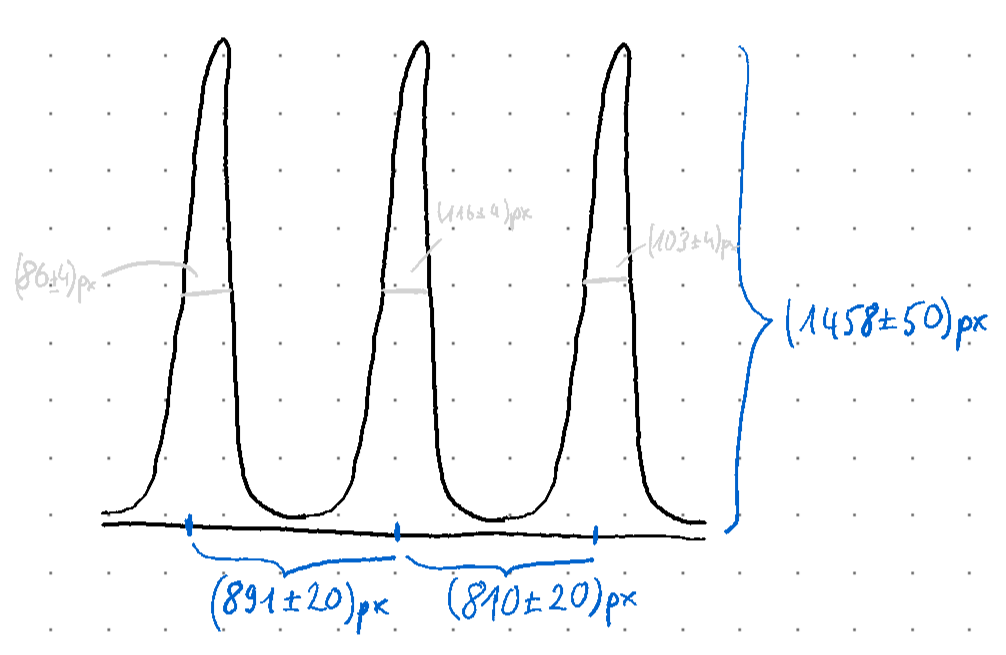
\includegraphics[width=0.5\textwidth]{Bilder/Bestimmung_Finesse_Skizze.png}
    }\\
   \caption{Bestimmen von $\Delta\omega_{\mathrm{FWHM}}$ und $\Delta\omega_{\mathrm{FSR}}$}
    \label{Bestimmen_Finesse_Fotostrecke}
\end{figure}
%\image{Oszi_entzerrt}{entzerrtes Bild zum Bestimmen von $\Delta\omega_{\mathrm{FWHM}}$ und $\Delta\omega_{\mathrm{FSR}}$}{.6}{Bilder/Bestimmung_Finesse.png}
Das Spektrum wurde in Form eines Fotos des Oszilloskopdisplays aufgenommen. Dieses Foto weist natürlich eine Parallaxe auf, d.h. das Display erscheint auf dem Foto verzerrt. Durch Anwenden einer linearen Transformation im Bildbearbeitungsprogramm GIMP kann das Bild entzerrt werden. Auf dem entzerrten Bild \ref{Bestimmen_Finesse_Fotostrecke} können pixelgenau die Abstände der Maxima und die FWHM-Breiten bestimmt werden. Da drei Maxima zu sehen sind, ergibt dies drei Werte für $\Delta\omega_{\mathrm{FWHM}}$ und zwei Werte für $\Delta\omega_{\mathrm{FSR}}$, aus denen je das arithmetische Mittel gebildet wird, dessen Unsicherheit über die empirische Standardabweichung (Wurzel der Varianz unter Berücksichtigung der Bessel-Korrektur) abgeschätzt werden kann.\\
Man erhält auf diese Weise die Werte $\Delta\overline\omega_{\mathrm{FWHM}}=(101\pm13)\mathrm{px}$ und $\Delta\overline\omega_{\mathrm{FSR}}=(850\pm50)\mathrm{px}$. Dabei ist $1\mathrm{px}\propto 1\mathrm s$, da das untersuchte Bild entzerrt ist. \\
Es ergibt sich somit für die Finesse:
\begin{equation}
F_1\equiv \frac{\Delta\overline\omega_{\mathrm{FSR}}}{\Delta\overline\omega_{\mathrm{FWHM}}}=8.4\pm1.5
\end{equation}
Alternativ kann die Finesse unter Benutzung von Gleichung \ref{finesse_theor} und den gemessenen Transmissivitäten der beiden halbdurchlässigen Spiegel des Resonators berechnet werden. Dabei wird Absorption in den Spiegeln vernachlässigt, d.h. $R_i+T_i=1,\ i\in\{1,2\}$. Weiterhin ist $T_i=\frac{U_i}{U_{\mathrm{ohne}\ \mathrm{Spiegel}}}$. Dann folgt nach \ref{finesse_theor} $F_2=27.5$ und mittels Gaußscher Fehlerfortpflanzung \begin{equation}
\Delta F_2 = \sqrt{\left(\frac{\partial F}{\partial U_1}\Delta U_1\right)^2+\left(\frac{\partial F}{\partial U_2}\Delta U_2\right)^2+\left(\frac{\partial F}{\partial U_{\mathrm{ohne}\ \mathrm{Spiegel}}}\Delta U_{\mathrm{ohne}\ \mathrm{Spiegel}}\right)^2}=1.6
\end{equation}
Somit ist $F_2>F_1$, was nicht überraschend ist, da $F_2$ die maximal erreichbare Finesse bei perfektem Justieren, d.h. bei idealem Spiegelabstand, bei exakt zueinander senkrechten Spiegeln und perfekter Position der Linse für Modenanpassung beschreibt.
\section{Zusammenfassung}
Das Vermessen des kollimierten und des fokussierten Laserstrahls hat gezeigt, dass das Intensitätsprofil in der Ebene senkrecht zur Ausbreitungsrichtung tatsächlich durch eine Gaußkurve beschrieben werden kann. Für einen fokussierten Laserstrahl konnte ferner die Verengung vor und die Auweitung der Strahlbreite nach dem Brennpunkt der Linse vermessen werden und damit gezeigt werden, dass der Verlauf gut durch eine Kurve beschrieben werden kann, wie sie die Gaußoptik vorhersagt. Ferner wurde der Gültigkeitsbereich der geometrischen Optik bei der Behandlung fokussierter Strahlen abgegrenzt. Oft genügt es bei der Konzeption eines optischen Aufbaus, die Propagation eines linearen Strahls in der paraxialen Näherung zu betrachten. Nur bei Bauelementen, bei denen der Wellencharakter des Lichtfeldes offensichtlich wird, bspw. nahe dem Fokuspunkt, beim Einkoppeln eines Strahls in eine Faser oder innerhalb eines Resonators aus gekrümmten Spiegeln, liefern die Methoden der geometrischen Optik keine physikalisch akkuraten Vorhersagen.
\newpage

\bibliography{literatur} 
\bibliographystyle{ieeetr}
\appendix


\section{Plots zur Vermessung des Strahldurchmessers}
\subsection{Ohne Linse (kollimiert)}
\plot{coll_z_75}{axiales Strahlprofil bei $z=75\mathrm{mm}$}{.8}{Messdaten Errorfunktion/Collimated_z_75.pdf}
\plot{coll_z_150}{axiales Strahlprofil bei $z=150\mathrm{mm}$}{.8}{Messdaten Errorfunktion/Collimated_z_150.pdf}
\plot{coll_z_250}{axiales Strahlprofil bei $z=250\mathrm{mm}$}{.8}{Messdaten Errorfunktion/Collimated_z_250.pdf}
\plot{coll_z_350}{axiales Strahlprofil bei $z=350\mathrm{mm}$}{.8}{Messdaten Errorfunktion/Collimated_z_350.pdf}
\subsection{Mit Linse (fokussiert)}
\plot{div_z_75}{axiales Strahlprofil bei $z=75\mathrm{mm}$}{.8}{Messdaten Errorfunktion/Divergent_z_75.pdf}
\plot{div_z_50}{axiales Strahlprofil bei $z=50\mathrm{mm}$}{.8}{Messdaten Errorfunktion/Divergent_z_50.pdf}
\plot{div_z_175}{axiales Strahlprofil bei $z=175\mathrm{mm}$}{.8}{Messdaten Errorfunktion/Divergent_z_175.pdf}
\plot{div_z_250}{axiales Strahlprofil bei $z=250\mathrm{mm}$}{.8}{Messdaten Errorfunktion/Divergent_z_250.pdf}
\plot{div_z_100}{axiales Strahlprofil bei $z=100\mathrm{mm}$}{.8}{Messdaten Errorfunktion/Divergent_z_100.pdf}
\plot{div_z_125}{axiales Strahlprofil bei $z=125\mathrm{mm}$}{.8}{Messdaten Errorfunktion/Divergent_z_125.pdf}
\section{Python-Skripte zur Auswertung}
\subsection{Bestimmung des axialen Strahlprofils}
%\large\textbf{Code 1 zu Plot TV5:}
\lstinputlisting{Messdaten Errorfunktion/Erf_plot.py}
\subsection{Bestimmung des Strahlprofils ohne Linse}
\lstinputlisting{Messdaten Errorfunktion/w_z_plot_coll.py}
\lstinputlisting{Messdaten Errorfunktion/w_z_plot_coll_without_M2.py}
\subsection{Bestimmung des Strahlprofils mit Linse}
\lstinputlisting{Messdaten Errorfunktion/w_z_plot_div.py}
\lstinputlisting{Messdaten Errorfunktion/w_z_plot_div_without_M2.py}
%\large\textbf{Code 2 zu Plot TV5:}
%\lstinputlisting{TV5_2.py}\newpage

\end{document}